\documentclass[review]{elsarticle}
%DIF LATEXDIFF DIFFERENCE FILE
%DIF DEL tmp-emotion_V0_2.tex   Fri Oct  4 01:07:24 2019
%DIF ADD tmp-emotion_V0_3.tex   Fri Oct  4 02:21:56 2019

\usepackage{lineno, hyperref}
% \usepackage[hyperfootnotes=false]{hyperref}
\usepackage{array, pbox}
\usepackage{mathtools}
\usepackage{caption}
\usepackage{graphicx}
\usepackage{subcaption}
\usepackage{CJKutf8}
\usepackage[page, title]{appendix}
% \usepackage{tablefootnote}
\usepackage{threeparttable}
\usepackage{etoolbox}
\appto\TPTnoteSettings{\footnotesize}
\usepackage[bottom]{footmisc}
\usepackage{siunitx}
\usepackage{ntheorem}
\theoremseparator{:}
\newtheorem{hyp}{Hypothesis}

\usepackage{multirow}
\usepackage[normalem]{ulem}
\useunder{\uline}{\ul}{}

%to have numbered 4th level sections 1.1.1.1
\setcounter{tocdepth}{4}
\setcounter{secnumdepth}{4}

% to remove period in 4th level sections 1.1.1.1
\makeatletter
\def\els@aparagraph[#1]#2{\elsparagraph[#1]{#2}}
\def\els@bparagraph#1{\elsparagraph*{#1}}
\makeatother
% to enter a newline after 4th level sections
\newcommand{\myparagraph}[1]{\paragraph{#1}\mbox{}\smallskip}


\modulolinenumbers[5]

\journal{Tourism Management}

%% APA style
\bibliographystyle{model5-names}\biboptions{authoryear}
%DIF PREAMBLE EXTENSION ADDED BY LATEXDIFF
%DIF UNDERLINE PREAMBLE %DIF PREAMBLE
\RequirePackage[normalem]{ulem} %DIF PREAMBLE
\RequirePackage{color}\definecolor{RED}{rgb}{1,0,0}\definecolor{BLUE}{rgb}{0,0,1} %DIF PREAMBLE
\providecommand{\DIFadd}[1]{{\protect\color{blue}\uwave{#1}}} %DIF PREAMBLE
\providecommand{\DIFdel}[1]{{\protect\color{red}\sout{#1}}}                      %DIF PREAMBLE
%DIF SAFE PREAMBLE %DIF PREAMBLE
\providecommand{\DIFaddbegin}{} %DIF PREAMBLE
\providecommand{\DIFaddend}{} %DIF PREAMBLE
\providecommand{\DIFdelbegin}{} %DIF PREAMBLE
\providecommand{\DIFdelend}{} %DIF PREAMBLE
%DIF FLOATSAFE PREAMBLE %DIF PREAMBLE
\providecommand{\DIFaddFL}[1]{\DIFadd{#1}} %DIF PREAMBLE
\providecommand{\DIFdelFL}[1]{\DIFdel{#1}} %DIF PREAMBLE
\providecommand{\DIFaddbeginFL}{} %DIF PREAMBLE
\providecommand{\DIFaddendFL}{} %DIF PREAMBLE
\providecommand{\DIFdelbeginFL}{} %DIF PREAMBLE
\providecommand{\DIFdelendFL}{} %DIF PREAMBLE
\newcommand{\DIFscaledelfig}{0.5}
%DIF HIGHLIGHTGRAPHICS PREAMBLE %DIF PREAMBLE
\RequirePackage{settobox} %DIF PREAMBLE
\RequirePackage{letltxmacro} %DIF PREAMBLE
\newsavebox{\DIFdelgraphicsbox} %DIF PREAMBLE
\newlength{\DIFdelgraphicswidth} %DIF PREAMBLE
\newlength{\DIFdelgraphicsheight} %DIF PREAMBLE
% store original definition of \includegraphics %DIF PREAMBLE
\LetLtxMacro{\DIFOincludegraphics}{\includegraphics} %DIF PREAMBLE
\newcommand{\DIFaddincludegraphics}[2][]{{\color{blue}\fbox{\DIFOincludegraphics[#1]{#2}}}} %DIF PREAMBLE
\newcommand{\DIFdelincludegraphics}[2][]{% %DIF PREAMBLE
\sbox{\DIFdelgraphicsbox}{\DIFOincludegraphics[#1]{#2}}% %DIF PREAMBLE
\settoboxwidth{\DIFdelgraphicswidth}{\DIFdelgraphicsbox} %DIF PREAMBLE
\settoboxtotalheight{\DIFdelgraphicsheight}{\DIFdelgraphicsbox} %DIF PREAMBLE
\scalebox{\DIFscaledelfig}{% %DIF PREAMBLE
\parbox[b]{\DIFdelgraphicswidth}{\usebox{\DIFdelgraphicsbox}\\[-\baselineskip] \rule{\DIFdelgraphicswidth}{0em}}\llap{\resizebox{\DIFdelgraphicswidth}{\DIFdelgraphicsheight}{% %DIF PREAMBLE
\setlength{\unitlength}{\DIFdelgraphicswidth}% %DIF PREAMBLE
\begin{picture}(1,1)% %DIF PREAMBLE
\thicklines\linethickness{2pt} %DIF PREAMBLE
{\color[rgb]{1,0,0}\put(0,0){\framebox(1,1){}}}% %DIF PREAMBLE
{\color[rgb]{1,0,0}\put(0,0){\line( 1,1){1}}}% %DIF PREAMBLE
{\color[rgb]{1,0,0}\put(0,1){\line(1,-1){1}}}% %DIF PREAMBLE
\end{picture}% %DIF PREAMBLE
}\hspace*{3pt}}} %DIF PREAMBLE
} %DIF PREAMBLE
\LetLtxMacro{\DIFOaddbegin}{\DIFaddbegin} %DIF PREAMBLE
\LetLtxMacro{\DIFOaddend}{\DIFaddend} %DIF PREAMBLE
\LetLtxMacro{\DIFOdelbegin}{\DIFdelbegin} %DIF PREAMBLE
\LetLtxMacro{\DIFOdelend}{\DIFdelend} %DIF PREAMBLE
\DeclareRobustCommand{\DIFaddbegin}{\DIFOaddbegin \let\includegraphics\DIFaddincludegraphics} %DIF PREAMBLE
\DeclareRobustCommand{\DIFaddend}{\DIFOaddend \let\includegraphics\DIFOincludegraphics} %DIF PREAMBLE
\DeclareRobustCommand{\DIFdelbegin}{\DIFOdelbegin \let\includegraphics\DIFdelincludegraphics} %DIF PREAMBLE
\DeclareRobustCommand{\DIFdelend}{\DIFOaddend \let\includegraphics\DIFOincludegraphics} %DIF PREAMBLE
\LetLtxMacro{\DIFOaddbeginFL}{\DIFaddbeginFL} %DIF PREAMBLE
\LetLtxMacro{\DIFOaddendFL}{\DIFaddendFL} %DIF PREAMBLE
\LetLtxMacro{\DIFOdelbeginFL}{\DIFdelbeginFL} %DIF PREAMBLE
\LetLtxMacro{\DIFOdelendFL}{\DIFdelendFL} %DIF PREAMBLE
\DeclareRobustCommand{\DIFaddbeginFL}{\DIFOaddbeginFL \let\includegraphics\DIFaddincludegraphics} %DIF PREAMBLE
\DeclareRobustCommand{\DIFaddendFL}{\DIFOaddendFL \let\includegraphics\DIFOincludegraphics} %DIF PREAMBLE
\DeclareRobustCommand{\DIFdelbeginFL}{\DIFOdelbeginFL \let\includegraphics\DIFdelincludegraphics} %DIF PREAMBLE
\DeclareRobustCommand{\DIFdelendFL}{\DIFOaddendFL \let\includegraphics\DIFOincludegraphics} %DIF PREAMBLE
%DIF END PREAMBLE EXTENSION ADDED BY LATEXDIFF

\begin{document}

\begin{frontmatter}

\title{Analyzing differences in satisfaction and dissatisfaction between Chinese and English-speaking customers of Japanese hotels with \DIFdelbegin \DIFdel{text-mining}\DIFdelend \DIFaddbegin \DIFadd{machine learning}\DIFaddend }

%% or include affiliations in footnotes:
\author[gidai]{Elisa Claire Alemán Carreón
\corref{mycorrespondingauthor}}
\ead{elisa.claire.aleman.carreon@gmail.com}
% \orcid{0000-0002-6437-0866}

\author[gidai]{Hugo Alberto Mendoza Espa\~na}
\ead{s173330@stn.nagaokaut.ac.jp}

\author[gidai]{Hirofumi Nonaka}
\ead{nonaka@kjs.nagaokaut.ac.jp}

\author[nagasaki]{Toru Hiraoka}
\ead{hiraoka@sun.ac.jp}

\address[gidai]{Nagaoka University of Technology, Nagaoka, Japan}
\address[nagasaki]{University of Nagasaki, Nagasaki, Japan}

\cortext[mycorrespondingauthor]{
Corresponding author%: \\
% Elisa Claire Alemán Carreón \\
% Mailing Address: P.C. 940-2033, Ribbon Nagaoka B104, 1128-3 Kaminozoki-machi, Nagaoka, Niigata, Japan \\
% Cell Phone: 080-9869-4756 \\
}

\begin{abstract}

Up until recently, most studies in tourist behavior have been biased for the Western world. With the increase of Chinese outbound tourists to countries across the globe, academic interest for this group has risen. \DIFdelbegin \DIFdel{However}\DIFdelend \DIFaddbegin \DIFadd{Increasing variation amongst clients means that managing hotels in a way that caters to their different tastes becomes more and more important. Despite this}\DIFaddend , cross-cultural studies of \DIFdelbegin \DIFdel{their differences with other }\DIFdelend \DIFaddbegin \DIFadd{differences between Asian and Western }\DIFaddend cultures are scarce and predate the current boom in the Chinese economy. This economical boom could change their expectations and experiences of Chinese customers, which would, in turn, influence their satisfaction and dissatisfaction with hotels. Additionally, most studies choose certain factors to be analyzed in their questionnaire, and this often is limited to managerial attributes of the hotel. With the spread of \DIFdelbegin \DIFdel{the use of }\DIFdelend Web 2.0 \DIFdelbegin \DIFdel{to write online reviews of hotels }\DIFdelend \DIFaddbegin \DIFadd{and online hotels reviews}\DIFaddend , a large amount of text data is available for research purposes. With \DIFdelbegin \DIFdel{text mining}\DIFdelend \DIFaddbegin \DIFadd{our method}\DIFaddend , we can use Shannon's entropy to automatically extract the satisfaction and dissatisfaction factors from very large data samples without interfering with the decision process of customers. This means that we can measure just how important are certain attributes of the hotel to customers, and whether those are managerial or environmental, that is, internal or external to the hotel. In our study, we performed a sentiment analysis using an SVM classifier and then measured the similarity value for satisfaction and dissatisfaction keyword frequency ranking lists using the Rank-biased Overlap measure, which can be used for top-weighted ranked lists with different elements and lengths. We found that Chinese customers prefer big and clean spaces and that Western customers are satisfied with friendly staff members. We also found that Chinese tourists are unsatisfied with the hotel being Chinese friendly with treatment and language and that Western customers are unsatisfied with rooms that they consider dirty, or that smell of cigarette. 


\medskip
\noindent\it{Highlights}
\begin{itemize}
    \item Chinese customers tend to prefer big and clean spaces but are unsatisfied with Chinese-friendliness.
    \item English-speaking customers are satisfied with friendly staff, but dislike rooms that are dirty or smell of cigarette.
    \item Both customer groups value the location of the hotel as a secondary factor for satisfaction.
    \item Both customer groups have concerns about the pricing of hotels (value for money).
    \item Satisfaction and dissatisfaction of customers come from managerial and environmental attributes of the hotel.
\end{itemize}

\end{abstract}

\begin{keyword}
Sentiment Analysis\sep Hotels and Lodging\sep Machine Learning\sep Chinese\sep English\sep Preferences
\end{keyword}

\end{frontmatter}

\linenumbers

\section{Introduction}\label{intro}

Recently, the Japanese economy has been more and more affected by an increase in inbound international tourism \cite[][]{jones2009} with a Year-on-Year Growth Rate of 19.3\% in 2017, with a total of \num[group-separator={,}]{28691073} inbound tourists that year \cite[][]{jnto2003-2019}. From this total, the tourist population was mostly Asian (86.14\%), with approximately a fourth of the total (25.63\%) coming from China. Western countries, counting English-speaking countries in addition to the whole of Europe make for 11.4\% of the total, with a 7.23\% of the total being countries where English is the official or the de facto national language. Specifically for Chinese tourists, the effect on international economies as well as the number of researchers interested in this phenomenon has been increasing as well \cite[][]{sun2017}. \DIFaddbegin \DIFadd{With these and other multicultural tourists populations, the tourist market is more and more diverse. Diversity in customers cultural backgrounds means that their expectations when staying at a hotel will also be varied. Hotel management therefore needs to cater to these different needs and expectations to increase their customers' satisfaction and maintain a good reputation generating positive word-of-mouth.
}\DIFaddend 

However, up until recently studies on social sciences, and that includes tourist behavior, have been performed using surveys on populations that could be culturally biased for the western world \cite[][]{nielsen2017, jones2010WEIRD, guaratne2009, hogan1978biases}. Those that do include Asian populations in their analysis, most commonly Chinese tourist behavior \cite[e.g.][]{liu2019, chang2010, dongyang2015}, and a few that compare Asian to western tourist behavior \cite[e.g.][]{choi2000}, are commonly survey or interview-based studies with small samples, which while valid can have its limitations. This creates a need for cross-cultural studies for the increasing Asian and Western tourist populations. It could be said that Westerners make for a smaller portion of the tourist population compared to Asians; however, according to \cite{choi2000}, Westerners are known as "long-haul" customers, spending more than 45\% of their budget on hotel lodging, compared to their Asian counterparts only spending 25\% of their budget on hotels. It is therefore important to study both Asian and Western tourist populations, their differences, and contrast the results with existing literature. 

With the advent of Web 2.0 and customer review websites, researchers realized the benefits of online reviews for research, and their importance for sales  \cite[][]{ye2009, basuroy2003}, customer consideration \cite[][]{vermeulen2009} and perception of services and products \cite[][]{browning2013}, among other effects of online interactions between customers \cite[e.g.][]{xiang2010, ren2019}. Consequentially, tourism research also began to use information collected online for data mining analysis, such as opinion mining \cite[e.g.][]{hu2017436}, predicting hotel demand from online traffic \cite[][]{yang2014}, recommender systems \cite[e.g.][]{loh2003}, and more. Data mining\DIFaddbegin \DIFadd{, machine learning }\DIFaddend and big data methodologies can increase the number of manageable samples from the hundred or so samples manually analyzed by researchers to the hundreds of thousands that are automatically analyzed by machines. This can not only help confirm existing theories but also lead to finding new patterns and to knowledge discovery \cite[][]{fayyad1996data}. 

In this study, we take advantage of the availability of enormous amounts of online reviews of Japanese hotels by both Chinese and Western English-speaking tourists populations. With this data, we can both confirm existing theories about their differences in behavior, as well as perform an exploration of the data to discover factors that could have been overlooked in the past. For this purpose, we use machine learning to automatically classify review sentences as positive or negative opinions of the hotel, and perform a statistical extraction of the topics that the customers of each population are most concerned about.


\section{Research objective}\label{research_objective}

The objective of this study is to determine the difference in preferences between Chinese-speaking and English-speaking customers of Japanese hotels using text-mining techniques. We aim to determine a quantitative measure of similarity (and therefore, difference) between the satisfaction and dissatisfaction factors of both customer groups using a Rank-biased Overlap measure. Furthermore, we \DIFdelbegin \DIFdel{aim to }\DIFdelend \DIFaddbegin \DIFadd{will }\DIFaddend measure if both customer groups have differences in priorities for the factors that are common to both groups. \DIFdelbegin \DIFdel{Furthermore, we aim to }\DIFdelend \DIFaddbegin \DIFadd{In addition, we also }\DIFaddend measure how much satisfaction and dissatisfaction of both customer groups are influenced by managerial attributes internal to the hotel, as well as environmental attributes external to the hotel. 

Aside from this, our proposal includes the use of large scale data from online hotel reviews in Chinese and English to study their differences in a statistical manner. In the past, survey-based studies have provided a theoretical background for a few specific tourist populations of a single culture or that travel with a single purpose; this means that cultural and language differences often cannot be observed in a single study. 

The difference in preferences that our study uncovers can become the focal point for making improvements in tourism and service industries, increase the satisfaction of customers, and influence them to write more satisfied online reviews that will in turn increase sales and attract new customers. 

\section{Theoretical background and hypothesis development}\label{theory_hypothesis}

\subsection{Customer satisfaction and dissatisfaction during hotel lodging}\label{theory_satisfaction}

Customer satisfaction in tourism has been analyzed since decades past, \cite{hunt1975} having defining customer satisfaction as the realization or overcoming of expectations towards the service. \cite{oliver1981} defined it as an emotional response to the provided services in retail and other contexts, and \cite{oh1996} reviewed the psychological processes of customer satisfaction for the hospitality industry. It is generally agreed upon that satisfaction and dissatisfaction stem from the individual expectations of the customer, and as such, \cite{engel1990} states that satisfaction and dissatisfaction are therefore influenced by each customer's background. This is why Western and Asian, specifically Chinese, customers can have very different factors of satisfaction and dissatisfaction since they have different backgrounds and cultures. These varying backgrounds will lead to varying expectations of the services that a hotel can provide for them, the experiences they want to have while staying at a hotel, and the level of comfort that they will have, from the moment that they choose the hotel throughout their stay. These contrasting expectations, in turn, will determine the contrasting factors of satisfaction and dissatisfaction for each kind of customer, as well as the order in which they prioritize them.
Therefore we propose our first and second hypothesis:

\begin{hyp}
\label{hyp:1}
Chinese and Western tourists have different \DIFaddbegin \DIFadd{priorities in hotel attributes that lead to their }\DIFaddend satisfaction and dissatisfaction\DIFdelbegin \DIFdel{factors}\DIFdelend .
\end{hyp}

\begin{hyp}
\label{hyp:2}
The common satisfaction and dissatisfaction factors identified for both Chinese and Western tourists will be placed at a different priority for each group.
\end{hyp}

Studies on customer satisfaction \cite[e.g.][]{truong2009, romao2014, wu2009} commonly use the Likert scale \cite[][]{likert1932technique} (e.g. 1 to 5 scale from strongly dissatisfied to strongly satisfied) to perform statistical analysis of which factors relate most to satisfaction on the same dimension as dissatisfaction \cite[e.g.][]{chan201518, choi2000}. This leads to correlation analyses (either multivariate or single variable ones) where one factor can lead to satisfaction, while it is implied that the lack of it can lead to dissatisfaction. However, a binary distinction (satisfied or dissatisfied) could allow us to analyze the factors that solely correlate to satisfaction, as well as exploring factors which are solely linked to dissatisfaction. There are fewer examples of this approach, but studies have also done this in the past \cite[e.g.][]{zhou2014}. While it is true that this method can decrease the extent to which we can analyze degrees of satisfaction or dissatisfaction, it has the benefit that it can be applied to a large sample of text data via automatic sentiment detection techniques using artificial intelligence. 

Previous research has also focused on factors that are controllable by the hotel managers and staff, i.e. hotel services, staff behavior, or facilities \cite[e.g.][]{shanka2004, choi2001}, while the satisfaction might also be influenced by factors that are uncontrollable by the hotel staff, such as surroundings, location, language immersion of the country as a whole, or of touristic destinations, as well as integration of the hotel with tours available nearby, among other factors that can play a part in the customers choice behavior and satisfaction. 
This leads to our third hypothesis:

\begin{hyp}
\label{hyp:3}
Satisfaction and dissatisfaction stems from both internal (managerial) and external (environmental) attributes of the hotel.
\end{hyp}

\subsection{Chinese and Western tourist behavior}\label{theory_zh_en}

% Asians vs Western behavior
In the past, tourist behavior analyzed from western samples and surveys was wrongly thought to be a representation of universal behavior across all cultures \cite[][]{nielsen2017, jones2010WEIRD, guaratne2009, hogan1978biases}. Recently, however, with the rise of Chinese outbound tourism, both academic researchers and businesses have decided to study Chinese tourist behavior \cite[][]{sun2017}. This results in several studies focusing on only the behavior of this subset of tourists. To this day, cross-cultural studies and analyses for Asian and Western tourists have been scarce. A few examples are \cite{choi2000}, where it was found that Western tourists visiting Hong Kong are satisfied more with room quality while Asians are satisfied with value for money; \cite{bauer1993changing}, where Westerners prefer the hotel health facilities while the Asian tourists were more inclined to enjoy the Karaoke facilities of hotels, and both groups tend to have high expectations about the overall facilities; and \cite{kim2000}, where American tourists were found to be individualistic and motivated by novelty, while Japanese tourists were found to be collectivist and motivated by prestige and family, with escape from routine and an increase in knowledge as a common motivator. 

One thing to note with the above cross-culture analyses is that they were performed before the year 2000. The current Chinese economy boom is making an increase in the influx of tourists, but the question that could be posed is whether that boom created a difference in the expectations of tourists and as such, in their satisfactions and dissatisfactions when traveling. Another note is that these studies were performed with questionnaires in places where it would be easy to locate tourists, i.e. airports. However, our study of online reviews takes the data that the hotel customers uploaded themselves.

% Universal behavior
Other more recent studies, perhaps recognizing that samples being comprised of people from Western industrialized countries aren't representative, have gone further and studied people from many countries in their samples, and performed a more universal and holistic (not cross-culture) analysis. \cite{choi2001}, for example, analyzed hotel guest satisfaction determinants in Hong Kong with surveys in English, Chinese and Japanese translations, with people from many countries in their sample. \cite{choi2001} found that staff service quality, room quality, and value for money were the top satisfaction determinants. For another example, \cite{Uzama2012} produced a typology for foreigners coming to Japan for tourism, without making distinctions for their culture, but their motivation in traveling in Japan. In another study, \cite{zhou2014} analyzed hotel satisfaction using English and Mandarin online reviews from guests staying in Hangzhou, China coming from many different countries. The general satisfaction score was noticed to be different in those countries, but a deeper cross-cultural analysis of the satisfaction factors wasn't performed. As a result of their research, \cite{zhou2014} thus found that customers are universally satisfied by welcome extras, dining environments, and special food services. 

% Western behavior 
Regarding Western tourist behavior, a few examples can tell us what to expect when analyzing our data. \cite{kozak2002} found that British and German tourists' satisfaction determinants while visiting Spain and Turkey were hygiene and cleanliness, hospitality, the availability of facilities and activities, and accommodation services. \cite{shanka2004} found that English-speaking tourists in Perth, Australia were most satisfied with staff friendliness, efficiency of check-in and check-out, restaurant and bar facilities and lobby ambiance. 

% Chinese behavior
Regarding outbound Chinese tourists, academic studies about Chinese tourists have increased \cite[][]{sun2017}. Different researchers have found that Chinese tourist populations have several specific attributes. According to \cite{ryan2001} and their study of Chinese tourists in New Zealand, Chinese tourists prefer nature, cleanliness, and scenery in contrast to experiences and activities. With some overlap, \cite{dongyang2015} studied Chinese tourists in the Kansai region of Japan and found that Chinese tourists are satisfied mostly with exploring the food culture of their destination, cleanliness, and staff. Studying Chinese tourists in Vietnam, \cite{truong2009} found that Chinese tourists are highly concerned with value for money. According to \cite{liu2019}, Chinese tourists tend to have harsher criticism when compared with other international tourists. And according to \cite{gao2017chinese}, who analyzed different generations of Chinese tourists and their connection to nature while traveling, Chinese tourists prefer nature overall, but the younger generations seem to do so less than their older counterparts. 

% Studies are not universal.
Although the studies focusing only on Chinese tourists or only on Western tourists have a narrow view, their theoretical contributions are valuable. We can see that depending on the study and the design of questionnaires, as well as the destinations, the results can vary greatly. Not only that, but while there seems to be some overlap in most studies, some factors are completely ignored in one study but not in the other. However, since our study uses data mining, the definition of each subject or factor is left for the hotel customers to decide en masse via their reviews (instead of being defined by the questionnaire). This means that the factors will be selected through statistical methods alone. This can open opportunities to find factors that the writers of this study would not have contemplated, or avoid enforcing a factor on the mind of reviewers by presenting them with a question that they didn't think of by themselves. In addition, this study could help us analyze the satisfaction and dissatisfaction factors cross-culturally and compare them with the existing literature.

\subsection{Data mining, knowledge discovery and sentiment analysis}\label{theory_data}

% Explain data mining and discovery of theory inside the data
In the current world, data is presented to us in larger and larger quantities. Today's data sizes were commonly only seen in very specialized large laboratories with supercomputers a couple of decades ago, but they are now common for market and managerial studies, independent university students and any scientist that can connect to the Internet. Such quantities of data are available to study now more than ever, but it would be impossible for researchers to parse all of this data by themselves. As \cite{fayyad1996data} summarizes, data by itself is unusable until it goes through a process of selection, preprocessing, transformation, mining, and evaluation, and only then it can be established as knowledge. With the tools available to us in the are of information science, algorithms can be used to detect patterns that would take researchers too long to recognize, which can be evaluated to generate knowledge. This process is called Knowledge Discovery in Databases. 

% Text mining 
Now, there are of course many sources of numerical data to be mined, but perhaps what is most available and interesting to managerial purposes is the resource of customers' opinions in text form. With the introduction of Web 2.0, a never before seen quantity of valuable information is being posted to the Internet at a staggering speed. Text mining then has been proposed more than a decade ago to utilize this data \cite[e.g.][]{rajman1998text,nahm2002text}, using what is called Natural Language Processing to parse language in a way that it can be analyzed by a computer, and improved on with the years. This has been used in the field of hospitality as well for many purposes, including satisfaction analysis from reviews \cite[e.g][]{berezina2016, xu2016, xiang2015, hargreaves2015, balbi2018}, social media's influence on travelers \cite[e.g.][]{xiang2010}, review summarization \cite[e.g.][]{hu2017436}, perceived value of reviews \cite[e.g][]{FANG2016498}, and even predicting hotel demand using web traffic data \cite[e.g][]{yang2014}.

% Sentiment Analysis
More than only analyzing patterns within the text, researchers have found how to determine the sentiment behind a statement based on speech patterns, statistical patterns, and other methodologies. This is called sentiment analysis, or opinion mining, and a precursor of this method was attempted for decades before \cite[][]{stone1966general}. With sentiment analysis, one could use patterns in the text to determine whether a sentence was being said with a positive opinion, a critical opinion, or even other ranges of emotions, depending on the thoroughness of the algorithm. Examples of sentiment analysis include ranking products through online reviews \cite[e.g][]{liu2017149, zhang2011}, predicting political poll results through opinions in Twitter \cite[][]{oconnor2010}, and so on. In the hospitality field, it has been used to classify reviewers' opinions of hotels in online reviews \cite[e.g.]{kim2017362, alsmadi2018}. 

% Data exploration
Because the methodology for finding patterns in the data is automatic and statistical in nature, it is both reliable, in that the algorithm will find a pattern by its nature, and unpredictable, in that because it has no intervention from the researchers in making questionnaires it can have different results from anything that the researchers could expect. This is why, much like actual mining, data mining is mostly exploratory in nature. One can never be sure that something can be found, but we can make predictions and estimates about where to find knowledge, and what kind of knowledge can be uncovered. 

In this study, we can predict that several things might occur. Our data could show satisfaction and dissatisfaction factors that are universal and it could also find strictly cultural preferences, but we expect that both of these options will present themselves. We can also assert that, if the previous literature is correct in their findings, we could arrive at very similar results, albeit using a database several orders of magnitude larger. We can also expect that, because of the lack of questionnaire design and freedom of users to record their pleasures and grievances, it is possible that we will discover patterns that were previously unnoticed by researchers.

\section{Methodology}\label{method}

We have extracted a large number of text reviews from a Chinese portal site \textit{Ctrip}\footnote{\label{ctrip}Ctrip: \href {www.ctrip.com/}{\path{www.ctrip.com/}}}, as well as the travel site \textit{TripAdvisor}\footnote{\label{tripadvisor}TripAdvisor: \href {www.tripadvisor.com/}{\path{www.tripadvisor.com/}}} and determined the most commonly used words that would contribute the most to positive and negative opinions in a review using Shannon's entropy to extract keywords from their vocabulary. These positive and negative keywords allow us to perform a Support Vector Machine based emotional classification of the reviews in large quantities, saving time and resources for the researchers. After classifying the sentences in the extracted reviews as emotionally positive or negative with an optimized SVM, we also observed their weight values in the machine, and the frequency of the terms in all of the reviews to extract the most utilized words in either kind of reviews. We show an overview of this methodology in Figure \ref{fig:method-overview} \cite[][]{Aleman2018ICAROB}.

\begin{figure}[bp]
\centering
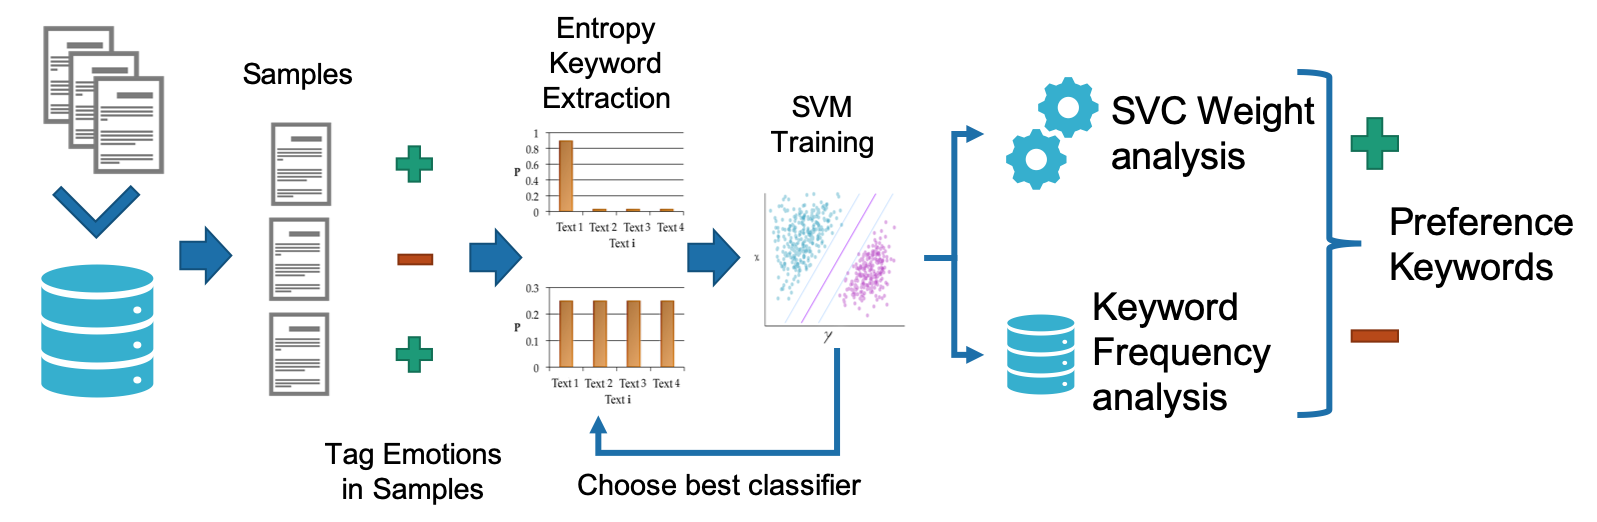
\includegraphics[width=\textwidth]{emotion-method-overview.png}
\caption{Overview of the methodology.}
\label{fig:method-overview}
\end{figure}

\subsection{Data collection}\label{datacollection}

In the data collection stage for Chinese reviews in \textit{Ctrip} a total of \num[group-separator={,}]{5938} review pages of hotels in Japan were collected. From these pages, we extracted a total of \num[group-separator={,}]{44177} reviews, which were comprised of \num[group-separator={,}]{572218} separate sentences. 

%DIF <  In our corpus, there were \num[group-separator={,}]{23443} different words used, from which \num[group-separator={,}]{2802} were noise characters.
\DIFdelbegin %DIFDELCMD < 

%DIFDELCMD < %%%
\DIFdelend In the TripAdvisor data collection, we collected data from \num[group-separator={,}]{21154} different hotels. In total, we collected \num[group-separator={,}]{295931} reviews in English, which we then separated into \num[group-separator={,}]{2697086} sentences using the \textit{gensim} python library. 

\subsection{Text processing}\label{textprocessing}

\DIFdelbegin \DIFdel{Because Chinese text doesn't have spaces, }\DIFdelend \DIFaddbegin \DIFadd{In order }\DIFaddend to parse Chinese words \DIFdelbegin \DIFdel{on their own }\DIFdelend \DIFaddbegin \DIFadd{and separate them }\DIFaddend we used the Stanford Word Segmenter \cite[][]{chang2008} program developed by the Stanford NLP Group\footnote{\label{stanfordnlp}The Natural Language Processing Group at Stanford University}. In the case of texts in English, however, only using spaces is not enough to correctly collect concepts. Because of variations and conjugations of words depending on the context and tense, a better segmentation is achieved by using lemmatization, which returns the dictionary form of each word. For this purpose, we used the \textit{gensim} library with the English texts.

\subsection{Sentiment analysis}\label{sentimentanalysis}

The sentiment analysis was performed using the methodology described in \cite{Aleman2018ICAROB}. \DIFdelbegin \DIFdel{A group of keywords is }\DIFdelend \DIFaddbegin \DIFadd{Keywords are }\DIFaddend determined by a \DIFdelbegin \DIFdel{calculation and }\DIFdelend comparison of Shannon's entropy \cite[][]{shannon1948} between two classes, and then \DIFdelbegin \DIFdel{the keywords }\DIFdelend \DIFaddbegin \DIFadd{they }\DIFaddend are used in \DIFdelbegin \DIFdel{a Support Vector Classifier }\DIFdelend \DIFaddbegin \DIFadd{an SVM }\DIFaddend \cite[][]{cortes1995}, optimizing \DIFdelbegin \DIFdel{the entropy comparison values }\DIFdelend \DIFaddbegin \DIFadd{keywords }\DIFaddend to select the best performing classifier. The selected \DIFdelbegin \DIFdel{classifier's feature }\DIFdelend \DIFaddbegin \DIFadd{SVM's }\DIFaddend keywords would then clearly represent the user preferences leading to positive and negative emotions. \DIFaddbegin \DIFadd{Examples of tagged sentences are shown in Table \ref{tab:training_examples}, and SVM performance results are shown in section \ref{apx:entropy_results}.
}\DIFaddend 

Shannon’\DIFdelbegin \DIFdel{s entropy, in the field of Information Theory, is defined to be the expected value of the information content in a signal. It is shown in formulas \ref{eq:H} and \ref{eq:lim_H}.
Using this value we can }\DIFdelend \DIFaddbegin \DIFadd{s entropy can be used to }\DIFaddend observe the probability distribution of each word inside the corpus. A word that is included in many documents will have a high entropy value for that set of documents. Opposite to this, a word appearing in only one document will have an entropy value of zero. 
\DIFdelbegin \DIFdel{We show this concept in Figure \ref{fig:entropygraphs}.
}\DIFdelend 

\DIFdelbegin \begin{displaymath}\DIFdel{%DIFDELCMD < \label{eq:H}%%%
H = - \sum_{i=1}^M }[\DIFdel{P \log_2 P}]
\end{displaymath}
%DIFAUXCMD
%DIFDELCMD < 

%DIFDELCMD < %%%
\begin{displaymath}\DIFdel{\label{eq:lim_H}
\lim_{P\to0+} P \log_2 P = 0
}\end{displaymath}
%DIFAUXCMD
%DIFDELCMD < 

%DIFDELCMD < \begin{figure}[bp]
%DIFDELCMD <     \centering
%DIFDELCMD <     \begin{subfigure}[b]{0.4\linewidth}
%DIFDELCMD <         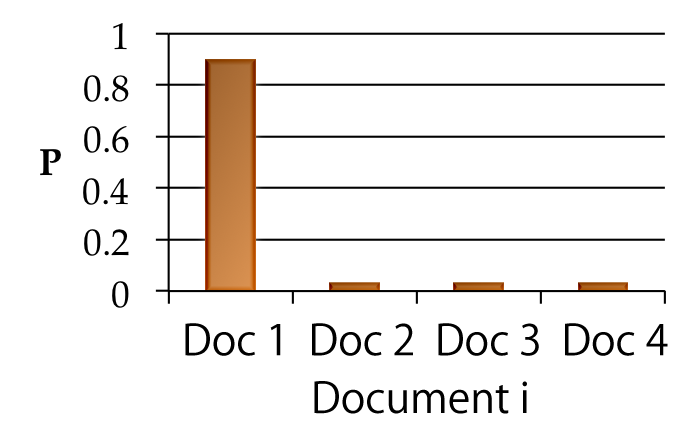
\includegraphics[width=\linewidth]{entropyzero.png}
%DIFDELCMD <         %%%
%DIFDELCMD < \caption{%
{%DIFAUXCMD
\DIFdelFL{Entropy close to zero.}}
    %DIFAUXCMD
%DIFDELCMD < \end{subfigure}
%DIFDELCMD <     \begin{subfigure}[b]{0.4\linewidth}
%DIFDELCMD <         \includegraphics[width=\linewidth]{entropyhigh.png}
%DIFDELCMD <         %%%
%DIFDELCMD < \caption{%
{%DIFAUXCMD
\DIFdelFL{High entropy}}
    %DIFAUXCMD
%DIFDELCMD < \end{subfigure}
%DIFDELCMD < %%%
%DIFDELCMD < \caption{%
{%DIFAUXCMD
\DIFdelFL{Probabilities of a word j being contained in a document i.}}
%DIFAUXCMD
%DIFDELCMD < \label{fig:entropygraphs}
%DIFDELCMD < \end{figure}
%DIFDELCMD < 

%DIFDELCMD < %%%
\DIFdel{To apply this logic, we retrieved 50 reviews as a sample of our corpus and with the collaboration of a group of 5 Chinese students, which were split into }\DIFdelend \DIFaddbegin \DIFadd{We tagged }\DIFaddend 159 \DIFdelbegin \DIFdel{sentences. We then tagged each sentence as the classes positive or negative depending on the emotion that the text conveyed, then calculated the entropy values for each word in relation to the set of sentences from each class. In the case of English reviews, we sampled 665 reviews and with the collaboration of English-speaking students manually tagged them by sentence, resulting in \num[group-separator={,}]{2357} tagged sentences . Words with higher entropy relating to the satisfaction set than to the dissatisfaction set by a factor of \(\alpha\) were determined to be keywords tied with satisfaction in Chinese reviews of hotels. This is shown in formula \ref{eq:entropy_pos}. Likewise, words with higher entropy for the dissatisfaction set than the satisfaction set by a factor of \(\alpha'\) were determined to be keywords tied to dissatisfaction in our texts. This is shown in formula \ref{eq:entropy_neg}. Examples of positive and negativesentences in English and Chinese are shown in the Appendix, in Table \ref{tab:training_examples}. }%DIFDELCMD < 

%DIFDELCMD < %%%
\begin{displaymath}\DIFdel{\label{eq:entropy_pos}
H_{P} > \alpha H_{N} %DIF <  \rightarrow satisfaction \: keyword
}\end{displaymath}
%DIFAUXCMD
%DIFDELCMD < 

%DIFDELCMD < %%%
\begin{displaymath}\DIFdel{\label{eq:entropy_neg}
H_{N} > \alpha' H_{P} %DIF <  \rightarrow dissatisfaction \: keyword
}\end{displaymath}
%DIFAUXCMD
%DIFDELCMD < 

%DIFDELCMD < %%%
\DIFdel{The mutually independent coefficients \(\alpha\) }\DIFdelend \DIFaddbegin \DIFadd{Chinese sentences }\DIFaddend and \DIFdelbegin \DIFdel{\(\alpha'\) were }\DIFdelend \DIFaddbegin \DIFadd{\num[group-separator={,}]{2357} English sentences as positive or negative. The entropy comparison factor was }\DIFaddend tested from 1.25 to 6 in intervals of 0.25. \DIFdelbegin \DIFdel{The result was 40 lists for each language, 20 for each emotional class. We trained a different Support Vector Classifier with each of the lists, and we chose the best performing lists for each emotional class and then combined the successful lists to train our best performing classifier. This resulted in a best performing positive emotion classifier (positive/non-positive) for each language.
}%DIFDELCMD < 

%DIFDELCMD < %%%
\DIFdel{For the performance tests, we used a 5-fold cross-validation \mbox{%DIFAUXCMD
\cite[][]{kohavi1995} }\hspace{0pt}%DIFAUXCMD
process in the Chinese reviews, and a 10-fold cross-validation process in the English reviews case, in which we calculated their F-measure \mbox{%DIFAUXCMD
\cite[][]{powers2011} }\hspace{0pt}%DIFAUXCMD
means and standard deviations. The number of \(k\)-folds was decided from the sample size. Table \ref{tab:svm_f1_zh} shows the lists that had the best performance results in the case of Chinese text and Table \ref{tab:svm_f1_en} shows the best performance results in English texts in the Appendix. 
}%DIFDELCMD < 

%DIFDELCMD < %%%
\DIFdel{We then used these best performing classifiers in the rest of the respective data to label positive emotion sentences in a binary manner. The sentences not belonging to the positive emotion class were considered to belong in the negative emotion class. This resulted in }\DIFdelend \DIFaddbegin \DIFadd{After classification, our data contained }\DIFaddend \num[group-separator={,}]{506452} positive Chinese sentences, \num[group-separator={,}]{65766} negative Chinese sentences, \num[group-separator={,}]{1288098} positive English sentences and \num[group-separator={,}]{1408988} negative English sentences. 

\subsection{SVM weight analysis}\label{svmweightsanalysis}

During the SVM learning algorithm, each point of data that is classified incorrectly causes a change in the weight vector to better classify new data correctly. These changes to the weight vector are strong for features that needed to be taken account of to classify with a minimal error, those \DIFdelbegin \DIFdel{contained in the support vectors, }\DIFdelend close to the separating hyperplane. Sequentially, the weight vector can be interpreted as a numerical representation of the effect each feature had for each class in the classification process. Below we show the formula for the weight vector (\ref{eq:svm_weight}).

\begin{equation}\label{eq:svm_weight}
w = \sum_{i=1}^N \alpha_i y_i x_i
\end{equation}

\subsection{Rank-biased Overlap}\label{rbo}

In order to compare the similarity between two ranked lists, most cases would call to action a statistical measure such as Kendall's \(\tau\). However, since the lists are not necessarily of the same length, or have necessarily the same contents, and are top-weighted (where the first rank is the most important to know, with less and less importance as the ranks continue), it is necessary to use another measure of similarity. \cite{webber2010similarity} proposed a Rank-biased Overlap measurement, which takes all of these factors into consideration \DIFaddbegin \DIFadd{when calculating a value from 0 to 1, where 0 means completely different lists and 1 means the two lists are an exact match}\DIFaddend . Because our Chinese keywords (their translations, at least) don't match our English keywords one to one, it is necessary to use this method. Webber's RBO produces 3 measurements: a minimum RBO, a residual RBO (from which one can know the maximum RBO), and an extrapolated RBO (where the list is assumed to continue in the same pattern of similarity towards infinity). The formula for the extrapolated RBO is shown in (\ref{eq:rbo_ext}), Where \(S\) and \(T\) are listings, \(d\) is their depth, \(k\) is their evaluation depth, \(p\) is a parameter that controls the top-weightedness of the lists (or it could be thought as \(1-p\) being the probability to stop looking at the next item in the list), and \(X\) being the overlap between the lists. The complete process is described at length by \cite{webber2010similarity}.

\begin{equation}\label{eq:rbo_ext}
RBO_{EXT}(S,T,p,k) = \frac{X_k}{k} \cdot p^k + \frac{1-p}{p} \sum_{d=1}^k{\frac{X_d}{d} \cdot p^d}
\end{equation}

\section{Data Analysis}\label{dataanalysis}

% WITHOUT PERCENTAGE
\subsection{Frequent keywords and their SVM weight values}\label{svmresults}

In order to understand the preferences of Chinese-speaking tourists and English-speaking tourists when lodging in Japan, we study both the frequency of the words they use in relation to the number of total reviews, and their weight in the SVM classifiers. Following that, to know the relevance of a keyword as a preference for each group, we observed the frequencies of each entropy-based keyword in our complete data set and their SVM weight value. The frequency of the keywords in the database shows the level of priority it has for customers, and the weight value allows us to observe the sentiment it relates to by its positive or negative sign. We ranked the keywords by frequency, and use their SVM weight for analyzing the related sentiment (positive weight means positive sentiment, and negative weight signifies negative sentiment). 

We observed the top 10 words with the highest frequencies for keywords that were linked by entropy to satisfaction and dissatisfaction in emotionally positive and negative statements to study and quantitatively rank the needs of Chinese customers, as shown in the Tables \ref{tab:pos_keys_zh} and \ref{tab:neg_keys_zh} (however, the latter does not have more than 7 keywords available); and for English-speaking customers, as shown in Tables \ref{tab:pos_keys_en} and \ref{tab:neg_keys_en}.

There were many more keywords than shown in most cases, however, and some showed to be high in weight but low in frequency. This could mean they were useful for classification (the emotional reaction is more extreme) but aren't as important a preference for users (there aren't many cases in that the keyword was applicable). In the appendix, Table \ref{tab:key_weights_zh} shows some keywords that have a relatively high weight value for both positive and negative extremes and their translations in the relevant context. In Table \ref{tab:key_weights_en} we show keywords for the English classifier with high weight values as well.

% Chinese_frequencies_svm_weight_positive_translations_matched.csv

\begin{table}[hbp] \centering
\caption{Top 10 frequently used positive Chinese keywords in satisfaction sentences.}
\label{tab:pos_keys_zh}
\begin{tabular}{|c|l|c|c|c|} \hline
\textbf{Word} & \multicolumn{1}{c|}{\textbf{Translation}} & \textbf{Frequency} & \textbf{SVC Weight} \\ \hline
% 1
\begin{CJK}{UTF8}{gbsn} 大 \end{CJK} 
    & big 
        & 15470 & 0.624 \\ \hline
% 2
\begin{CJK}{UTF8}{gbsn} 干净 \end{CJK} 
    & clean 
        & 12166 & 0.638 \\ \hline
% 3
\begin{CJK}{UTF8}{gbsn} 早餐 \end{CJK} 
    & breakfast 
        & 10575 & 0.495 \\ \hline
% 4
\begin{CJK}{UTF8}{gbsn} 推荐 \end{CJK} 
    & recommendation 
        & 8752 & 0.495 \\ \hline
% 5
\begin{CJK}{UTF8}{gbsn} 环境 \end{CJK} 
    & \begin{tabular}[c]{@{}l@{}}
    environment
    \end{tabular} 
        & 8694 & 0.248 \\ \hline
% 6
\begin{CJK}{UTF8}{gbsn} 周边 \end{CJK} 
    & periphery 
        & 8456 & 0.495 \\ \hline
% 7
\begin{CJK}{UTF8}{gbsn} 近 \end{CJK} 
    & close
        & 8372 & 0.028 \\ \hline
% 8
\begin{CJK}{UTF8}{gbsn} 交通 \end{CJK} 
    & transportation
        & 8264 & 0.586 \\ \hline
% 9
\begin{CJK}{UTF8}{gbsn} 附近 \end{CJK} 
    & nearby
        & 6619 & 0.495 \\ \hline
% 10
\begin{CJK}{UTF8}{gbsn} 地铁 \end{CJK} 
    & subway
        & 5386 & 0.180 \\ \hline
\end{tabular}
\end{table}

% Chinese_frequencies_svm_weight_negative_translations_matched.csv

\begin{table}[hbp] \centering
\caption{Frequently used negative Chinese keywords in dissatisfaction sentences.}
\label{tab:neg_keys_zh}
\begin{tabular}{|c|l|c|c|} \hline
\textbf{Word} & \multicolumn{1}{c|}{\textbf{Translation}} & \textbf{Frequency} & \textbf{SVC Weight} \\ \hline
% 1
\begin{CJK}{UTF8}{gbsn} 价格 \end{CJK} 
    & price 
        & 7636 & -1.505 \\ \hline
% 2
\begin{CJK}{UTF8}{gbsn} 地理 \end{CJK} 
    & geography 
        & 2238 & -0.812 \\ \hline
% 3
\begin{CJK}{UTF8}{gbsn} 中文 \end{CJK} 
    & Chinese language 
        & 1410 & -0.714 \\ \hline
% 4
\begin{CJK}{UTF8}{gbsn} 陈旧 \end{CJK} 
    & old-fashioned 
        & 698 & -0.000 \\ \hline
% 5
\begin{CJK}{UTF8}{gbsn} 距离 \end{CJK} 
    & distance 
        & 349 & 0 \\ \hline
% 6
\begin{CJK}{UTF8}{gbsn} 老 \end{CJK} 
    & old 
        & 311 & 0 \\ \hline
% 7
\begin{CJK}{UTF8}{gbsn} 华人 \end{CJK} 
    & Chinese person 
        & 16 & -0.238 \\ \hline
\end{tabular}
\end{table}


% Hugo_1_SVM_Combined_p1.5_n4.25_c2_Frequency_counts_posinega_subject-only.csv


\begin{table}[hbp]
\centering
\caption{Top 10 positive English keywords in satisfaction sentences.}
\label{tab:pos_keys_en}
\begin{tabular}{|l|c|c|}
\hline
\multicolumn{1}{|c|}{\textbf{Word}} & \textbf{Frequency} & \textbf{SVC Weight} \\ \hline
% 1
staff & 138677 & 0.537 \\ \hline
% 2
clean & 105971 & 1.886 \\ \hline
% 3
location & 103151 & 0.842 \\ \hline
% 4
helpful & 63558 & 1.999 \\ \hline
% 5
comfortable & 62793 & 1.724 \\ \hline
% 6
friendly & 57307 & 1.199 \\ \hline
% 7
recommend & 51433 & 1.158 \\ \hline
% 8
train & 45148 & -0.000 \\ \hline
% 9
free & 42084 & 0.734 \\ \hline
% 10
subway & 38354 & 1.951 \\ \hline
\end{tabular}
\end{table}

% Hugo_1_SVM_Combined_p1.5_n4.25_c2_Frequency_counts_posinega_subject-only.csv

\begin{table}[hbp]
\centering
\caption{High negative weight English keywords in dissatisfaction sentences.}
\label{tab:neg_keys_en}
\begin{tabular}{|l|c|c|}
\hline
\multicolumn{1}{|c|}{\textbf{Word}} & \textbf{Frequency} & \textbf{SVC Weight} \\ \hline
% 1
pricey & 3809 & -1.614 \\ \hline
% 2
carpet & 3683 & -0.507 \\ \hline
% 3
slow & 3177 & -1.281 \\ \hline
% 4
dirty & 2943 & -1.275 \\ \hline
% 5
uncomfortable & 2942 & -2.423 \\ \hline
% 6
stain & 2787 & -1.886 \\ \hline
% 7
cigarette & 2468 & -0.435 \\ \hline
% 8
curtain & 2032 & -0.224 \\ \hline
% 9
paper & 2029 & -0.503 \\ \hline
% 10
renovation & 1898 & -0.548 \\ \hline
\end{tabular}
\end{table}

\subsection{Rank-biased Overlap}\label{rboresults}

In order to calculate the similarity between the ranked lists shown in Tables \ref{tab:pos_keys_zh} and \ref{tab:pos_keys_en}, and the lists in Tables \ref{tab:neg_keys_zh} and \ref{tab:neg_keys_en}, we calculated the extrapolated Rank-biased Overlap between the English keyword lists and the English translation of the Chinese keyword lists at different cutoff points. Additionally, we prepared and modified the lists so that words that are similar but would not overlap otherwise would overlap in this analysis. For example, in the English keyword lists, the word is 'pricey' while in the Chinese keywords it is translated as 'price', and as such, it was changed to 'pricey' to match the English keywords. The results of this are shown in Table \ref{tab:rbo}. In the case of Chinese dissatisfaction keywords, which is only comprised of 7 keywords, the list remains complete in all cutoff points \DIFdelbegin \DIFdel{bigger than 7, and then it is cut at the cutoff point of }\DIFdelend \DIFaddbegin \DIFadd{except }\DIFaddend 5. Since the RBO measure can work regardless of the length of each list, this is not a problem in its calculation.

% Please add the following required packages to your document preamble:
% \usepackage{multirow}
\begin{table}[hbp]
\centering
\caption{RBO results between Chinese and English ranked keyword lists, \(p=0.9\).}
\label{tab:rbo}
\begin{tabular}{|l|c|r|}
\hline
\multicolumn{1}{|c|}{\textbf{List cutoff}} & \textbf{Emotion} & \(RBO_{EXT}\) \\ \hline
\multirow{2}{*}{None}   & Satisfaction      & 0.265 \\ \cline{2-3} 
                        & Dissatisfaction   & 0.299 \\ \hline
\multirow{2}{*}{Top 20} & Satisfaction      & 0.265 \\ \cline{2-3} 
                        & Dissatisfaction   & 0.293 \\ \hline
\multirow{2}{*}{Top 10} & Satisfaction      & 0.266 \\ \cline{2-3} 
                        & Dissatisfaction   & 0.285 \\ \hline
\multirow{2}{*}{Top 5}  & Satisfaction      & 0.221 \\ \cline{2-3} 
                        & Dissatisfaction   & 0.321 \\ \hline
\end{tabular}
\end{table}

\section{Results}\label{results}

\DIFdelbegin \subsection{\DIFdel{Chinese tourists' satisfaction and dissatisfaction keywords}}
%DIFAUXCMD
\addtocounter{subsection}{-1}%DIFAUXCMD
%DIFDELCMD < 

%DIFDELCMD < %%%
\DIFdel{Analyzing satisfaction keywords of Chinese hotel reviews from Table \ref{tab:pos_keys_zh}, we found that the most relevant subjects Chinese customers perceive positively are cleanliness and size, very possibly of the room they had stayed in. There is also the possibility that reviewers were praising, in general, the cleanliness of Japan’s environment, streets without litter, potable water and their culture of respecting spaces. Our results also indicate that the closeness of the hotel to scenic places is highly preferred by Chinese customers. Lower in the list of priorities, other positive factors that come into play when Chinese tourists choose a hotel to stay are the location in relation to public transport availability (such as the subway); and as mentioned before, environments, such as gardens or parks nearby; and services nearby, like places to go shopping. 
}%DIFDELCMD < 

%DIFDELCMD < %%%
\DIFdel{One key component we found in Chinese customer preferences is the inclusion of breakfast within the hotel. This can be inferred from the high frequency with which this keyword was included in the sentences emotionally classified as positive. While other food-related words were extracted, most of them were general in nature, like “food” or “eating”, and in a lower ranking. In contrast, the word “breakfast”, which is referring to a specific time and very possibly its inclusion in the hotel commodities, was very frequently used in positive texts compared to other food-related words. 
}%DIFDELCMD < 

%DIFDELCMD < %%%
\DIFdel{Regarding dissatisfaction keywords in Table \ref{tab:neg_keys_zh}, we found that the most frequently criticized aspect of Japanese hotels was the price. Another important negative factor can be the availability or lack thereof of Chinese translations. Chinese customers can feel lost when they don't understand directions or instructions, either written or spoken; however, according to our data, most customers can be thought to have complained about written translations. Another dissatisfaction factor is the word 'old', which can be referring to the age of the building, or the general design and look of the place being old-fashioned.
}%DIFDELCMD < 

%DIFDELCMD < %%%
\DIFdel{We can assert that Chinese customers value the room quality over transportation availability, that they are interested in included breakfast with the hotel stay, that they are concerned with value for money and the availability of Chinese language translations to have an easier time in the accommodation.
}%DIFDELCMD < 

%DIFDELCMD < %%%
\subsection{\DIFdel{English-speaking tourists' satisfaction and dissatisfaction keywords}}
%DIFAUXCMD
\addtocounter{subsection}{-1}%DIFAUXCMD
%DIFDELCMD < 

%DIFDELCMD < %%%
\DIFdel{The most important satisfaction keyword in English reviews (see Table \ref{tab:pos_keys_en}) is 'staff', while lower in the list we can also observe 'helpful' and 'friendly', possibly referring to the staff as well, and since Japan is famous for its customer service culture, this is not unexpected. Next on the list, we can observe they value cleanliness, but a few more items in the list are regarding the location of the hotel, and possibly the availability of nearby transportation, such as the subway or train. We can also observe that the word 'free' is present there, which after observing a few examples in the database, we concluded that it relates to the free amenities in a hotel room, such as cosmetics, soaps, coffee, tea, and so on.
}%DIFDELCMD < 

%DIFDELCMD < %%%
\DIFdel{The negative keywords of dissatisfied customer reviews (see Table \ref{tab:neg_keys_en}) reveal an interesting picture. While the most used keyword is also related to the price of the hotels, most of the keywords are related to the hygiene of the hotel, namely dirty carpets, stains, cigarette smell in the room or curtains, and so on. We can also observe that the word 'renovation' is written lower in the list, as well as the word 'paper'. After observation of the samples, it is often used with the expression 'paper-thin walls', which could mean the customers can hear their neighbors easily. Regarding the word 'renovation', some cities in Japan (e.g. Osaka) are currently going under a large number of renovations, which are also extending to the hotel facilities. Customers staying in places in renovation or near a renovation construction can be expected to wake up to construction noises, have their view obstructed by metal bars, and other unpleasant experiences. Another keyword there is 'slow', which upon inspection of example reviews, we concluded that it reflects the speed of the Internet connection in the hotel rooms.
}%DIFDELCMD < 

%DIFDELCMD < %%%
\DIFdel{We can assert that English-speaking tourists value staff friendliness and location convenience concerning transport, but are concerned about any kind of decline in room quality both visually and regarding the smell and air quality, being quick to judge any sort of remains of cigarette smell.
}%DIFDELCMD < 

%DIFDELCMD < %%%
\DIFdelend \subsection{Comparison of Chinese and English-speaking tourists' preferences}

%DIF <  USE Results from Rank-biased Overlap (full list) experiment results_p_0.9_cutoff_10.txt
\DIFdelbegin %DIFDELCMD < 

%DIFDELCMD < %%%
\DIFdelend The extrapolated Rank-biased Overlap (shown in Table \ref{tab:rbo}) ranged from 0.221 to 0.265 in satisfaction lists\DIFdelbegin \DIFdel{at different cutoff points}\DIFdelend , and from 0.285 to 0.321 in the dissatisfaction lists, which are low similarity values \DIFaddbegin \DIFadd{(\(RBO_{EXT} < 0.5\))}\DIFaddend . This means that, while there is some similarity, the preferences are fundamentally different if we consider them as top-weighted, that is, the first elements are the most important in the lists, and therefore in their similarity measurement as well. This confirms our hypothesis \ref{hyp:1}, that the \DIFaddbegin \DIFadd{priorities for }\DIFaddend satisfaction and dissatisfaction \DIFdelbegin \DIFdel{factors }\DIFdelend are different for Chinese and English-speaking tourists. 

From observation, however, we can assert that both Chinese and English-speaking tourists in Japan have different priorities, but consider the location of the hotel and the availability of transport nearby, such as subway or trains, as a secondary but still important point in their satisfaction of a hotel. The Chinese customers are primarily satisfied with the room quality in spaciousness and cleanliness, while the English-speaking customers are easily upset by any lack of cleanliness and smoke smell from cigarettes. English-speaking tourists on the other hand value staff friendliness over room quality when considering their satisfaction. 

The lists for Chinese and English-speaking tourists are quite different, but if we compare the lists, we find that 'clean', 'recommend', 'subway' and 'price' are common \DIFdelbegin \DIFdel{satisfaction and dissatisfaction }\DIFdelend factors to both customer groups\DIFdelbegin \DIFdel{accordingly. Furthermore, their }\DIFdelend \DIFaddbegin \DIFadd{. Their }\DIFaddend place in the ranked list is the \DIFdelbegin \DIFdel{same for 'clean', 'subway' and 'price', making }\DIFdelend \DIFaddbegin \DIFadd{exact same for most of them, and }\DIFaddend only 1 out of 4 factors \DIFdelbegin \DIFdel{different in priority. }\DIFdelend \DIFaddbegin \DIFadd{is different in rank. Furthermore, when arranging both lists by eliminating all uncommon elements, the lists become identical with an RBO of 1.0 for both satisfaction and dissatisfaction lists. }\DIFaddend This means hypothesis \ref{hyp:2} is rejected \DIFdelbegin \DIFdel{, where even }\DIFdelend \DIFaddbegin \DIFadd{(\(RBO_{EXT} > 0.5\)), where }\DIFaddend the similar aspects in both customer groups were hypothesized to be different in their priority.

We also can observe some keywords that aren't considered by their counterparts. For example, Chinese tourists are very satisfied with breakfast inclusion, while English-speaking customers are satisfied with free amenities. On the other hand, English-speaking customers mentioned tobacco smell in many reviews, while it wasn't statistically identified as a problem at all for their Chinese counterparts.

As to the top 10 satisfaction and dissatisfaction keywords themselves we can observe whether they are attributes internal to the hotel, that is, managerial in nature, or external to it, environmental in nature. \DIFdelbegin \DIFdel{For the satisfaction factors of Chinese-speaking tourists, 30\% of the keywords are managerial factors, while 60\% of them are environmental factors ('recommendation' is not counted as either). On the other hand, for the satisfaction factors of English-speaking tourists, 60\% of them are managerial, while 30\% of them are environmental. Now, for the dissatisfaction factors of Chinese customers, 71.4\% of them are managerial while the remaining 28.6\% of them are environmental. On the other hand, a 100\% of the dissatisfaction factors for English-speaking customers are managerial in nature. }\DIFdelend We can see these results in Table \ref{tab:hyp3}. The interpretation of these keywords is shown in the Appendix in Tables \ref{tab:man_env_pos} and \ref{tab:man_env_neg}.

% Please add the following required packages to your document preamble:
% \usepackage{multirow}
% \usepackage{graphicx}
\begin{table}[]
\caption{Managerial and Environmental nature of the most frequently used keywords}
\label{tab:hyp3}
\resizebox{\textwidth}{!}{%
\begin{tabular}{|c|c|r|r|r|}
\hline
\textbf{Emotion} & \textbf{Customer group} & \multicolumn{1}{c|}{\textbf{\begin{tabular}[c]{@{}c@{}}Managerial\\ Factors\end{tabular}}} & \multicolumn{1}{c|}{\textbf{\begin{tabular}[c]{@{}c@{}}Environmental\\ Factors\end{tabular}}} & \multicolumn{1}{c|}{\textbf{Unidentified}} \\ \hline
\multirow{2}{*}{Satisfaction} & Chinese speakers & 30\% & 60\% & 10\% \\ \cline{2-5} 
 & English speakers & 60\% & 30\% & 10\% \\ \hline
\multirow{2}{*}{Dissatisfaction} & Chinese speakers & 71.4\% & 28.6\% & 0\% \\ \cline{2-5} 
 & English speakers & 100\% & 0\% & 0\% \\ \hline
\end{tabular}%
}
\end{table}

For our purposes, hypothesis \ref{hyp:3} states that the satisfaction and dissatisfaction factors would stem from both managerial and environmental attributes to the hotel. This is confirmed for all but one list. The exception is the English-speaking tourists' top 10 dissatisfaction factors, which are all managerial in nature. However, this is only regarding the top 10 items in the list, and lower in the list there are some environmental factors.

\section{Discussion}\label{discussion}

\subsection{Chinese tourists - A big, clean space, and Chinese friendly}\label{disc:zh}

We found that Chinese tourists are satisfied mostly by a big and clean space provided by the Japanese hotels. From further inspection, we also find that while this is mostly relating to the rooms, there are many references to the public bathing facilities in the hotel. In Japan, there is what is called \textit{sent\=o}, which are artificially made public bathing facilities, on occasions including saunas and baths with special qualities. On the other hand, there are natural hot springs, called \textit{onsen}, which can be either bathing in the natural source of the water, or using the hot-spring water in artificially made bath facilities. It is a Japanese custom and culture that all customers use the facilities after cleaning themselves in a shower and go into the baths without any clothes. This can be a cultural shock for many tourists, but still, this is an important attraction for many.

From these two first ranking keywords, we can assert that 'Room Quality' is the most important satisfaction factor for Chinese customers. This means that Chinese tourists have an expectation of spaciousness and cleanliness when coming to Japan, be it by reputation, previous experiences, or cultural backgrounds. Whichever is the case, it appears that Chinese tourists are satisfied, which means their expectations regarding the rooms are being met. We can compare this result with previous literature, where traveling Chinese tourists choose their destination based on several factors, including cleanliness, nature, architecture, and scenery \cite[][]{ryan2001}. This other few factors found in previous literature could be linked to the keyword 'environment' as well.

\DIFaddbegin \DIFadd{One key component we found in Chinese customer preferences is the inclusion of breakfast within the hotel. This can be inferred from the high frequency with which this keyword was included in the sentences emotionally classified as positive. While other food-related words were extracted, most of them were general in nature, like “food” or “eating”, and in a lower ranking. In contrast, the word “breakfast”, which is referring to a specific time and very possibly its inclusion in the hotel commodities, was very frequently used in positive texts compared to other food-related words. 
}

\DIFaddend Moreover, Chinese tourists have expectations about the treatment towards the Chinese visitors that aren't being met. Be it Chinese language pamphlets, Chinese texts on instructions for the hotel room and it's appliances and features (T.V. channels, Wi-Fi setup, etc), or just the treatment towards Chinese people, it seems that their expectations are not being met. This is natural, since traveling in a strange land without knowledge of the language can be a daunting experience. \cite{ryan2001} also found that communication difficulties was one of the main reasons Chinese customers would give for not visiting again. 

\subsection{Western tourists - A friendly face, and absolutely clean}\label{disc:en}

From the satisfaction factors of English-speaking tourists, we can see that at least 3 words relate to staff friendliness and services. The word 'staff' is the most frequently used word for satisfied customers, while 'helpful' and 'friendly' follow it lower in the list at the 4th and 6th place. Japan is famous for their customer service all over the world. Staff members are trained to speak in \textit{sonkeigo}, or 'respectful language', one of the most formal of the Japanese formality syntaxes. They are also trained to bow with different depths depending on the situation, where a light bow could be used to say 'Please, allow me to guide you', and a deep bow to apologize for any inconvenience the customer could have, with a very respectful apology as well. This is all very different from Westerner experiences and while it could be a culture shock to some, it is mostly seen positively. After all, Japanese staff treats all customers in this respectful manner, but for some customers, this could very well be the best they have been treated until that moment. We can also see that \cite{kozak2002} and \cite{shanka2004} have also found that hospitality and staff friendliness is an important determinant in the satisfaction of Western tourists. \DIFaddbegin \DIFadd{On another note, we can also observe that the word 'free' is present in the satisfaction keywords, which after observing a few examples in the database, we concluded that it relates to the free amenities in a hotel room, such as cosmetics, soaps, coffee, tea, and so on. 
}\DIFaddend 

However, we can see from the rest of the keywords in combination that most of the dissatisfaction with Japanese hotels stems from a lack of hygiene and room cleanliness. Where Chinese customers were completely satisfied, English-speaking customers have found many places unacceptable to their standards. The most common complaint regarding cleanliness was about the carpet, followed by complaints about stains, and cigarette stench in the curtains. \cite{kozak2002} also found that hygiene and cleanliness were important satisfaction determinants for Western tourists. However, in the previous literature, this was linked merely to satisfaction. In comparison, our research uncovered that it is mostly linked to dissatisfaction and that westerners could be said to have high standards of hygiene when compared to their Chinese counterparts. \DIFaddbegin \DIFadd{Aside from cleanliness, we can also observe the word 'renovation' is written lower in the list, as well as the word 'paper'. After observation of the samples, it is often used with the expression 'paper-thin walls', which could mean the customers can hear their neighbors easily. Regarding the word 'renovation', some cities in Japan (e.g. Osaka) are currently going under a large number of renovations, which are also extending to the hotel facilities. Customers staying in places in renovation or near a renovation construction can be expected to wake up to construction noises, have their view obstructed by metal bars, and other unpleasant experiences. Another keyword there is 'slow', which upon inspection of example reviews, we concluded that it reflects the speed of the Internet connection in the hotel rooms.
}\DIFaddend 

\subsection{Price, the common enemy}\label{disc:price}

For both customer groups, the main reason for dissatisfaction is price, which can be interpreted as a concern for value for money. A paper studying Chinese tourists found that they had this concern \cite[][]{truong2009}, but our results indicate that in the case of Japanese hotels, this is less of a cultural attribute, and has more to do with the pricing of hotels overall. The tourists coming to Japan could be both experienced travelers or first-time travelers, but the fact is that their expectation of the price for hotels was lower than what they found in Japan. In general, Japan is an expensive place to visit, which could have an impact in this placement in the ranking. 

\subsection{Location, location, location}\label{disc:location}

The location of the hotel, closeness to subway and public transport, and availability of nearby shops were observed to be of importance to both Chinese and English-speaking tourists. While it wasn't the priority for either of them, we can assert that the location of the hotel is a secondary but still important point in their satisfaction of a hotel. However, since this is an external factor to the management of the hotel, it is not often considered in literature. Upon inspection of examples from the data, we found that most customers were satisfied if the hotel was nearby to at least two other subjects: subway or train, and convenience stores. 

Japan is a country with a particular public transport system. The rush hour makes for a subway filled to the brim with people in suits making their commute, and trains and subway stations in Tokyo create a confusing map for an outside observer. Buses are also available, although less used than the rail systems in the big cities. These three are particularly affordable in price. Then there are the more expensive transports, such as the bullet train \textit{shinkansen} for traveling across the country, and taxis. Taxis in Japan are a luxury compared to other countries. Where in less developed countries the taxi is the cheap method of transport of choice, in Japan, taxis are made to provide a high-quality experience, with a matching price. This means that for tourists, subway availability and a good map or plan to travel the city are of utmost necessity.

Japanese convenience stores, on the other hand, are also famous worldwide for their convenience. From drinks and snacks to full meals, copy and scanning machines, alcohol, cleaning supplies, personal hygiene items, underwear, towels, and so on, Japanese convenience stores are a haven for the traveler in need. If some trouble occurred, or a traveler forgot to pack a certain item, it is almost sure that they can find it here.

Therefore, considering both transport systems and nearby shops, Japanese hotels have to choose carefully their location from the moment that they are constructed. While not a top priority, this is a universal factor for both customer groups and it can be an instant way to generate positive reviews.

\subsection{Tobacco, what's that smell?}\label{disc:tobacco}

A main concern for Western tourists was the smell of tobacco in their room. Upon manual inspection of a sample of reviews with this keyword, we found that it was often the case that the room was advertised as non-smoking, and yet the smell permeated the room and curtains. Another common complaint was that there wasn't any non-smoking facilities available at all, to begin with. This can completely ruin some customers' stay, and give a bad impression for review writers, which can lower the number of future customers.

However, in comparison, Chinese customers seem to not be bothered by this at all. We consulted studies involving the use of tobacco in different countries. Previous research states that 49 - 60\% of Chinese men (and 2.0 - 2.8\% of women) currently smoke or have smoked before, taken from a sample of \num[group-separator={,}]{170000} Chinese adults in 2013-2014, which is high compared to many English-speaking countries \cite[][]{zhang2019tobacco, who2015tobacco}.

Japan itself has a polarized view on smoking, and despite being one of the world's largest tobacco markets, its use has been decreasing in recent years. While smoking in public spaces is prohibited in some wards of Tokyo (namely Chiyoda, Shinjuku, and Shibuya), it is generally only urged and not mandatory to have smoking restrictions in restaurants, bars, hotels, and public areas. However, there are many places where 'smoking rooms' are available to keep the smoke to an enclosed area and avoid bothering others. Despite this, businesses, especially those who cater to certain kinds of customers, will generally be discouraged from having smoking restrictions if they want to keep their clientele. If Japanese hotels want to cater to all kinds of customers, Western and Asian alike, they must provide spaces without tobacco smell. After all, even if it doesn't bother some customers, the lack of smell would not bother any existing customers. 

\subsection{Managerial vs. Environmental satisfaction}\label{disc:hyp3}

As we stated in section \ref{theory_satisfaction}, previous research is focused mostly on internal or managerial attributes of the hotel and their influence on customer satisfaction. For example, staff behavior, facilities, commodities, amenities, and appliances that can be improved within the hotel \cite[e.g.][]{shanka2004, choi2001}. However, external or environmental attributes, such as location of the hotel relative to public transport and shops, language immersion of the country, noise pollution, weather, and so on, are not usually analyzed in satisfaction studies. Because our study left the satisfaction factors to be decided statistically via customers' online reviews, we can see in their priorities the amount of importance that those environmental or managerial attributes can have. 

From Table \ref{tab:hyp3} and appendix Tables \ref{tab:man_env_pos} and \ref{tab:man_env_neg}, we can see that in regards to satisfaction, Chinese tourists have a 60\% of keywords of an environmental nature (namely 'environment','periphery','close','transportation','nearby', and 'subway'), while the remaining 30\% is managerial in nature. However, those words are all concentrated at the top of the list ('big','clean','breakfast'). In comparison, English speakers are mostly satisfied with managerial attributes of the hotel, with keywords such as 'staff', 'clean', 'helpful', and 'free' to name a few. English-speaking customers also have managerial attributes at the very top of their list. This means that in order to satisfy both Chinese and Western tourists, a hotel has the ability to improve in ways that will attract more customers in the future. If it was the other way around and the satisfaction was to be related more with environmental attributes, hotels would have to compete solely on their location. Similarly, most of the dissatisfaction is caused by issues that could be solved with improved management. Of course, this could be staff training (perhaps in language), hiring professional cleaning services for rooms with smoke smells, or improving the bedding, all of which can be costly. However, if hotels want to attract more and more customers, this paper provides a good guideline for which factors to consider first, and which ones will be best suited to which customer groups.

\section{Limitations}\label{limitations}

This paper is not without its limitations. We analyzed keywords of satisfaction and dissatisfaction statistically based on whether they appeared on satisfied reviews or not. Following that, we performed observations of sentences with those words, in an attempt to understand the context that these words were being used in. However, because of the large number of sentences in our data being analyzed, we could not perform a complete analysis of the context of these sentences across the database. Another limitation is that a big portion of the Asian tourists coming to Japan are Taiwanese and Korean, of which we couldn't do an analysis because of team members not knowing those languages. Aside from that, because of the anonymous nature of the data, further typology analysis couldn't be made (for example, Chinese men and women of different ages, or the same for Westerners).

\section{Conclusion and Future Work}\label{conclusion}

In this study, with the purpose to analyze the differences in satisfaction and dissatisfaction between Chinese and English-speaking customers of Japanese hotels, we extracted keywords from their online reviews to the portal sites \textit{Ctrip} and \textit{TripAdvisor} using Shannon's entropy calculations; then we used these keywords for sentiment classification via a Support Vector Classifier. We then measured the Rank-biased Overlap of the top 10 most frequently used keywords in satisfied and dissatisfied sentences in Chinese and English reviews to find their similarity (or lack thereof). We obtained values ranging from 0.221 to 0.265 in satisfaction lists and from 0.285 to 0.321 in dissatisfaction lists at different cutoff points. These are low values \DIFaddbegin \DIFadd{(\(RBO_{EXT} < 0.5\))}\DIFaddend , so we can assert that the preferences of Chinese and English-speaking tourists are different, confirming our hypothesis \ref{hyp:1}. 

We then measured the similarity in ranking from the words that were common satisfaction or dissatisfaction factors for both Chinese and English speakers, and found that from the four words that were common amongst both groups ('clean', 'recommend', 'subway' and 'price'), \DIFdelbegin \DIFdel{only one of the words ('recommend') had a different place in the ranking of the lists for either group}\DIFdelend \DIFaddbegin \DIFadd{their ranking when isolated from the uncommon elements in both lists was identical, resulting in an RBO of 1.0}\DIFaddend . This means our hypothesis \ref{hyp:2} is rejected \DIFaddbegin \DIFadd{(\(RBO_{EXT} > 0.5\))}\DIFaddend , and that the common ground within both customer groups is also similar in ranking.

Lastly, we measured the amount of satisfaction and dissatisfaction factors that were referring to managerial attributes of a hotel (that it can be changed via managerial decisions without relocating) or environmental attributes of the hotel (things like location, closeness to shops or public transport). We found that both are included in the satisfaction and dissatisfaction of both customer groups, confirming our hypothesis \ref{hyp:3}. We also found that most of the Western customer satisfaction (60\% of the top 10 words) and dissatisfaction (100\% of the top 10 words) stems from managerial attributes of the hotel, while environmental attributes only make for a smaller portion of the factors (30\% of the top 10 satisfaction keywords). In the case of Chinese customer satisfaction, the top of the list was managerial in nature (30\% of the top 10 words) and a bigger portion, although lower in ranking, was environmental in nature (60\%). For Chinese customer dissatisfaction, however, 71.4\% of the keywords were managerial in nature, while the other 28.6\% were environmental in nature.

Our results and discussion can be utilized as a guideline for managerial decisions when considering Chinese and Western tourists, and we can observe their stark differences, as well as their common attributes. In future work we plan to investigate further into this topic, extending our data set and researching for different trends for different regions of Japan and in different kinds of hotels, as well as between customers traveling alone or in groups, for fun or work. Another point for the future of this study is to use word clusters with similar meanings instead of single words. 

\section*{Acknowledgments}

During our research, \DIFdelbegin \DIFdel{apart from the group of Chinese students that collaborated with the training data and emotion tagging process, }\DIFdelend we received the commentary and discussion necessary to understand certain cultural aspects that could influence the interpretation of the data \DIFdelbegin \DIFdel{, from empirical and anecdotal Chinese sources, as well as collaboration in understanding the meaning behind the words we extracted }\DIFdelend by our dear colleagues, whom we would like to show gratitude to, Mr. Zhou Liangyuan, Ms. Fan Min and Ms. Eerdengqiqige. \DIFaddbegin \DIFadd{We would also like to show gratitude to Ms. Jajus Aleksandra, from whom we also received notes on the editing and commentary on the content of our manuscript.
}\DIFaddend 

\medskip

Funding: This work was supported by the Japan Construction Information Center Foundation (JACIC).

\medskip

Declarations of interest: none

\clearpage

%DIF <  \section*{References}
\DIFaddbegin \section*{\DIFadd{References}}
\DIFaddend 

\bibliography{bibfile-emotion}

\clearpage

\appendixpage
\appendix

\section{Sentiment analysis training data examples}\DIFaddbegin \label{apx:sentences_ex}
\DIFaddend 

% Please add the following required packages to your document preamble:
% \usepackage{multirow}
% \usepackage{graphicx}
% \usepackage[normalem]{ulem}
% \useunder{\uline}{\ul}{}
\begin{table}[hbp]
\centering
\caption{Examples of positive and negative sentences used for training SVM}
\label{tab:training_examples}
\resizebox{\textwidth}{!}{%
\begin{tabular}{|c|c|l|}
\hline
\textbf{Language} & \textbf{Emotion} & \textbf{Sentences} \\ \hline
\multirow{4}{*}{Chinese} & \multirow{2}{*}{Positive} & \begin{tabular}[c]{@{}l@{}}\begin{CJK}{UTF8}{gbsn} 酒店 的 服务 很 好 和 我 住 过 的 所有 日本 酒店 一样 各 种 隐形 服务 非常 厉害 \end{CJK}\\ (translated as: "The service of the hotel is very good. \\ All the services of the Japanese hotels I have stayed in are extremely good.")\end{tabular} \\ \cline{3-3} 
 &  & \begin{tabular}[c]{@{}l@{}} \begin{CJK}{UTF8}{gbsn} 有 一 个 后门 到 地铁站 非常 近 周边 也 算 方便 酒店 服务 和 卫生 都 很 好 \end{CJK} \\ (translated as: "There is a back door to the subway station very close to it. \\ The surrounding area is also convenient hotel service and health are very good")\end{tabular} \\ \cline{2-3} 
 & \multirow{2}{*}{Negative} & \begin{tabular}[c]{@{}l@{}} \begin{CJK}{UTF8}{gbsn} 酒店 旁边 很 荒凉 连个 便利 店 都 要 走 很远 \end{CJK} \\ (translated as: "The hotel is very bleak, \\ and you have to go very far to go to the nearest convenience store.")\end{tabular} \\ \cline{3-3} 
 &  & \begin{tabular}[c]{@{}l@{}} \begin{CJK}{UTF8}{gbsn} 唯一 不 足 是 价格 太高 \end{CJK} \\ (translated as: "The only negative is that the price is too high.")\end{tabular} \\ \hline
\multirow{4}{*}{English} & \multirow{2}{*}{Positive} & It was extremely clean, peaceful and the hotel Hosts made us feel super welcome \\ \cline{3-3} 
 &  & \begin{tabular}[c]{@{}l@{}}Location is very good, close to a main road with a subway station, a bakery,\\  a 7 eleven and a nice restaurant that is not too expensive but serves good food\end{tabular} \\ \cline{2-3} 
 & \multirow{2}{*}{Negative} & \begin{tabular}[c]{@{}l@{}}The only downside: our room was labeled 'non-smoking' \\ but our duvet reeked of smoke.\end{tabular} \\ \cline{3-3} 
 &  & A bit pricey though \\ \hline
\end{tabular}%
}
\end{table}


\section{Entropy keyword extraction experiment results}\DIFaddbegin \label{apx:entropy_results}
\DIFaddend 

As explained in section \ref{sentimentanalysis}, we performed experiments with different entropy values to extract keywords from the vocabulary. Then we chose the best performing classification machine based on those keywords as shown in the Tables \ref{tab:svm_f1_zh} and \ref{tab:svm_f1_en}. We also performed experiments to choose the best value of the parameter C used in SVC. C is a constant that affects the optimization process when minimizing the error of the separating hyperplane. Low values of C give some freedom of error, which minimizes false positives, but depending on the data it can increase false negatives. Inversely, high values of C will likely result in minimal false negatives, but a possibility of false positives. 

% Please add the following required packages to your document preamble:
% \usepackage{graphicx}
\begin{table}[hbp]
\centering
\caption{Best performing SVC 5-fold cross-validation Chinese text classifiers.}
\label{tab:svm_f1_zh}
\begin{tabular}{|l|l|l|l|l|}
\hline
\textbf{Keyword List} & \textbf{\begin{tabular}[c]{@{}l@{}}Classifier \\ emotion\end{tabular}} & \textbf{C} & \begin{tabular}[c]{@{}l@{}}\(F_1\) \\ \(\mu\)\end{tabular} & \begin{tabular}[c]{@{}l@{}}\(F_1\) \\ \(\sigma\)\end{tabular} \\ \hline
\begin{tabular}[c]{@{}l@{}}Satisfaction keywords \\ (\(\alpha=2.75\))\end{tabular} & \begin{tabular}[c]{@{}l@{}}Satisfaction \end{tabular} & 2.5 & 0.91 & 0.01 \\ \hline
\begin{tabular}[c]{@{}l@{}}Negative keywords \\ (\(\alpha'=3.75\))\end{tabular} & \begin{tabular}[c]{@{}l@{}}Dissatisfaction \end{tabular} & 0.5 & 0.67 & 0.11 \\ \hline
\begin{tabular}[c]{@{}l@{}}\textbf{Combined} \\ (\(\alpha\)=2.75, \(\alpha'\)=3.75)\end{tabular} & \textbf{\begin{tabular}[c]{@{}l@{}}Satisfaction\end{tabular}} & \textbf{0.5} & \textbf{0.95} & \textbf{0.01} \\ \hline
\end{tabular}
\end{table}

\begin{table}[hbp] \centering
\caption{Best performing SVC 10-fold cross-validation English text classifiers.}
\label{tab:svm_f1_en}
\begin{tabular}{|l|l|l|l|l|}
\hline
Keyword List & \begin{tabular}[c]{@{}l@{}}Classifier \\ emotion\end{tabular} & C & \begin{tabular}[c]{@{}l@{}}\(F_1\) \\ \(\mu\)\end{tabular} & \begin{tabular}[c]{@{}l@{}}\(F_1\) \\ \(\sigma\)\end{tabular} \\ \hline
\begin{tabular}[c]{@{}l@{}}Satisfaction keywords \\ (\(\alpha=1.5\))\end{tabular} & \begin{tabular}[c]{@{}l@{}}Satisfaction\end{tabular} & 1.75 & 0.82 & 0.02 \\ \hline
\begin{tabular}[c]{@{}l@{}}Dissatisfaction keywords \\ (\(\alpha'=4.25\))\end{tabular} & \begin{tabular}[c]{@{}l@{}}Dissatisfaction\end{tabular} & 3 & 0.80 & 0.03 \\ \hline
\begin{tabular}[c]{@{}l@{}}\textbf{Combined} \\ (\(\alpha\)=1.5, \(\alpha'\)=4.25)\end{tabular} & \textbf{\begin{tabular}[c]{@{}l@{}}Satisfaction\end{tabular}} & \textbf{2} & \textbf{0.83} & \textbf{0.02} \\ \hline
\end{tabular}
\end{table}

\section{Keywords with high SVM weights regardless of frequency}\DIFaddbegin \label{apx:keywords_weights}
\DIFaddend 

There were many more keywords than shown in Tables \ref{tab:pos_keys_en} and \ref{tab:neg_keys_en}. Some showed to be high in weight but low in frequency. This could mean they were useful for classification but aren't as important a preference for users. Table \ref{tab:key_weights_zh} shows some keywords that have a relatively high weight value for both positive and negative extremes and their translations in the relevant context. In Table \ref{tab:key_weights_en} we show keywords for the English classifier with high weight values as well.

\begin{table}[hbp] \centering
\caption{Chinese keywords with high SVM weight values regardless of frequency.}
\label{tab:key_weights_zh}
\begin{tabular}{|>{\centering\arraybackslash}m{3em}|m{10em}|>{\centering\arraybackslash}m{7em}|>{\centering\arraybackslash}m{5em}|} \hline
\textbf{Word} & \multicolumn{1}{c|}{\textbf{Translation}} & \textbf{Entropy List} & \textbf{SVC Weight} \\ \hline
\begin{CJK}{UTF8}{gbsn} 地方 \end{CJK} 
    & region, local 
        & Positive 
        & 1.343 \\ \hline
\begin{CJK}{UTF8}{gbsn} 干净 \end{CJK} 
    & clean 
        & Positive 
        & 0.638 \\ \hline
\begin{CJK}{UTF8}{gbsn} 大 \end{CJK} 
    & big, wide 
        & Positive 
        & 0.624 \\ \hline
\begin{CJK}{UTF8}{gbsn} 交通 \end{CJK} 
    & traffic, transportation 
        & Positive 
        & 0.586 \\ \hline
\begin{CJK}{UTF8}{gbsn} 热情 \end{CJK} 
    & cordial, kindness 
        & Positive 
        & 0.495 \\ \hline
\begin{CJK}{UTF8}{gbsn} 周边 \end{CJK} 
    & periphery 
        & Positive 
        & 0.495 \\ \hline
\begin{CJK}{UTF8}{gbsn} 景色 \end{CJK} 
    & scenery 
        & Positive 
        & 0.495 \\ \hline
\begin{CJK}{UTF8}{gbsn} 推荐 \end{CJK} 
    & recommendation 
        & Positive 
        & 0.495 \\ \hline
\begin{CJK}{UTF8}{gbsn} 日本 \end{CJK} 
    & Japan 
        & Positive 
        & 0.495 \\ \hline
\begin{CJK}{UTF8}{gbsn} 早餐 \end{CJK} 
    & breakfast 
        & Positive 
        & 0.495 \\ \hline
\begin{CJK}{UTF8}{gbsn} 附近 \end{CJK} 
    & nearby 
        & Positive 
        & 0.495 \\ \hline
\begin{CJK}{UTF8}{gbsn} 中文 \end{CJK} 
    & Chinese text 
        & Negative 
        & -0.714 \\ \hline
\begin{CJK}{UTF8}{gbsn} 地理 \end{CJK} 
    & geography 
        & Negative 
        & -0.812 \\ \hline
\begin{CJK}{UTF8}{gbsn} 价格 \end{CJK} 
    & price 
        & Negative 
        & -1.505 \\ \hline
\end{tabular}
\end{table}

\begin{table}[hbp]
\centering
\caption{English keywords with high SVM weight values regardless of frequency.}
\label{tab:key_weights_en}
\begin{tabular}{|l|c|c|}
\hline
\multicolumn{1}{|c|}{\textbf{Word}} & \multicolumn{1}{c|}{\textbf{\begin{tabular}[c]{@{}c@{}}Entropy\\ List\end{tabular}}} & \multicolumn{1}{c|}{\textbf{SVC Weight}} \\ \hline
bathhouse & Positive & 2.000 \\ \hline
museum & Positive & 2.000 \\ \hline
meeting & Positive & 1.997 \\ \hline
subway & Positive & 1.951 \\ \hline
cozy & Positive & 2.000 \\ \hline
convenience & Positive & 1.888 \\ \hline
clean & Positive & 1.886 \\ \hline
comfortable & Positive & 1.724 \\ \hline
dirty & Negative & -1.275 \\ \hline
policy & Negative & -1.463 \\ \hline
prepay & Negative & -1.517 \\ \hline
pricey & Negative & -1.614 \\ \hline
sticky & Negative & -2.000 \\ \hline
\end{tabular}
\end{table}

\section{Managerial and Environmental keywords}\DIFaddbegin \label{apx:man_env}
\DIFaddend 

\DIFdelbegin \DIFdel{In section }\DIFdelend \DIFaddbegin \DIFadd{As explained on }\DIFaddend \ref{disc:hyp3}, we \DIFdelbegin \DIFdel{discussed how satisfaction of the customer can come both from managerial attributes of the hotel, as well as environmental attributes. We }\DIFdelend identified the nature of each keyword in the top 10 lists of both satisfaction and dissatisfaction for Chinese and English-speaking tourists and summarized them in Table \ref{tab:hyp3}. The detailed identification of each keyword is shown in Tables \ref{tab:man_env_pos} and \ref{tab:man_env_neg} below.

% Please add the following required packages to your document preamble:
% \usepackage{graphicx}
% \usepackage[normalem]{ulem}
% \useunder{\uline}{\ul}{}
\begin{table}[hbp]
\centering
\caption{Hotel attribute types for the top 10 satisfaction keywords}
\label{tab:man_env_pos}
\resizebox{\textwidth}{!}{%
\begin{tabular}{|l|l|l|r|r|}
\cline{1-2} \cline{4-5}
\multicolumn{1}{|c|}{\textbf{\begin{tabular}[c]{@{}c@{}}Hotel Attribute\\ Type\end{tabular}}} & \multicolumn{1}{c|}{\textbf{\begin{tabular}[c]{@{}c@{}}Chinese satisfaction\\ keywords (translation)\end{tabular}}} & \multicolumn{1}{c|}{\textbf{}} & \multicolumn{1}{c|}{\textbf{\begin{tabular}[c]{@{}c@{}}English satisfaction\\ keywords\end{tabular}}} & \multicolumn{1}{c|}{\textbf{\begin{tabular}[c]{@{}c@{}}Hotel Attribute\\ Type\end{tabular}}} \\ \cline{1-2} \cline{4-5} 
managerial & big &  & staff & managerial \\ \cline{1-2} \cline{4-5} 
managerial & clean &  & clean & managerial \\ \cline{1-2} \cline{4-5} 
managerial & breakfast &  & location & environmental \\ \cline{1-2} \cline{4-5} 
unidentified & recommendation &  & helpful & managerial \\ \cline{1-2} \cline{4-5} 
environmental & environment &  & comfortable & managerial \\ \cline{1-2} \cline{4-5} 
environmental & periphery &  & friendly & managerial \\ \cline{1-2} \cline{4-5} 
environmental & close &  & recommend & unidentified \\ \cline{1-2} \cline{4-5} 
environmental & transportation &  & train & environmental \\ \cline{1-2} \cline{4-5} 
environmental & nearby &  & free & managerial \\ \cline{1-2} \cline{4-5} 
environmental & subway &  & subway & environmental \\ \cline{1-2} \cline{4-5} 
\end{tabular}%
}
\end{table}

% Please add the following required packages to your document preamble:
% \usepackage{graphicx}
\begin{table}[hbp]
\centering
\caption{Hotel attribute types for the top 10 dissatisfaction keywords}
\label{tab:man_env_neg}
\resizebox{\textwidth}{!}{%
\begin{tabular}{lll|r|r|}
\cline{1-2} \cline{4-5}
\multicolumn{1}{|c|}{\textbf{\begin{tabular}[c]{@{}c@{}}Hotel Attribute\\ Type\end{tabular}}} & \multicolumn{1}{c|}{\textbf{\begin{tabular}[c]{@{}c@{}}Chinese dissatisfaction\\ keywords (translation)\end{tabular}}} & \multicolumn{1}{c|}{\textbf{}} & \multicolumn{1}{c|}{\textbf{\begin{tabular}[c]{@{}c@{}}English dissatisfaction\\ keywords\end{tabular}}} & \multicolumn{1}{c|}{\textbf{\begin{tabular}[c]{@{}c@{}}Hotel Attribute\\ Type\end{tabular}}} \\ \cline{1-2} \cline{4-5} 
\multicolumn{1}{|l|}{managerial} & \multicolumn{1}{l|}{price} &  & pricey & managerial \\ \cline{1-2} \cline{4-5} 
\multicolumn{1}{|l|}{environmental} & \multicolumn{1}{l|}{geography} &  & carpet & managerial \\ \cline{1-2} \cline{4-5} 
\multicolumn{1}{|l|}{managerial} & \multicolumn{1}{l|}{Chinese language} &  & slow & managerial \\ \cline{1-2} \cline{4-5} 
\multicolumn{1}{|l|}{managerial} & \multicolumn{1}{l|}{old-fashioned} &  & dirty & managerial \\ \cline{1-2} \cline{4-5} 
\multicolumn{1}{|l|}{environmental} & \multicolumn{1}{l|}{distance} &  & uncomfortable & managerial \\ \cline{1-2} \cline{4-5} 
\multicolumn{1}{|l|}{managerial} & \multicolumn{1}{l|}{old} &  & stain & managerial \\ \cline{1-2} \cline{4-5} 
\multicolumn{1}{|l|}{managerial} & \multicolumn{1}{l|}{Chinese person} &  & cigarette & managerial \\ \cline{1-2} \cline{4-5} 
 &  &  & curtain & managerial \\ \cline{4-5} 
 &  &  & paper & managerial \\ \cline{4-5} 
 &  &  & renovation & managerial \\ \cline{4-5} 
\end{tabular}%
}
\end{table}



\end{document}
